% This is text associated with the open textbook "Open Electromagnetics"
% See immediately below for author, date
% This work is licensed under the Creative Commons Attribution-ShareAlike 4.0 International License. (CC BY SA 4.0) 
% To view a copy of the license, visit http://creativecommons.org/licenses/by-sa/4.0/

%ORB TITLE Loss Tangent
%ORB AUTHOR 0        # S.W. Ellingson, Virginia Tech (ellingson@vt.edu)
%ORB DATE 20191119   # yyyymmdd
%ORB ABSTRACT  

\label{m0132_Loss_Tangent} % <-- Must match name of this file and module directory name.  Don't mess with this!
\index{loss tangent|(}

In Section~\ref{m0128_Wave_Equations_Lossy_Regions}, we found that the effect of loss due to non-zero conductivity $\sigma$ could be concisely quantified using the ratio 
%
\begin{equation}
\frac{\epsilon''}{\epsilon'} = \frac{\sigma}{\omega\epsilon}
\label{m0132_eratio}
\end{equation}
%
where $\epsilon'$ and $\epsilon''$ are the real and imaginary components of the complex permittivity $\epsilon_c$, and $\epsilon'\triangleq\epsilon$.  In this section, we explore this relationship in greater detail.

Recall Ampere's law in differential (but otherwise general) form:
\index{Ampere's law!general form}
%
\begin{equation}
\nabla \times {\bf H} = {\bf J} + \frac{\partial}{\partial t}{\bf D}
\label{m0132_ACL2}
\end{equation}
%
The first term on the right is conduction current, whereas the second term on the right is displacement current.
\index{displacement current}
In the phasor domain, differentiation with respect to time ($\partial/\partial t$) becomes multiplication by $j\omega$.  Therefore, the phasor form of Equation~\ref{m0132_ACL2} is
%
\begin{equation}
\nabla \times \widetilde{\bf H} = \widetilde{\bf J} + j\omega\widetilde{\bf D}
\end{equation}
%
Also recall that $\widetilde{\bf J}=\sigma\widetilde{\bf E}$ and that $\widetilde{\bf D}=\epsilon\widetilde{\bf E}$. Thus,
%
\begin{equation}
\nabla \times \widetilde{\bf H} = \sigma\widetilde{\bf E} + j\omega\epsilon\widetilde{\bf E}
\end{equation}
%
Interestingly, the total current is the sum of a real-valued conduction current and an imaginary-valued displacement current.
This is shown graphically in Figure~\ref{m0132_fLossTan}.
%
\begin{figure}[b!]
\begin{center}
\pdftooltip{{  % note double braces
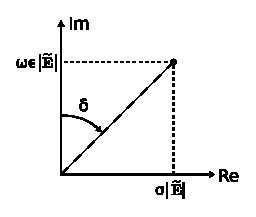
\includegraphics[width=0.8\columnwidth]{modules/m0132_fLossTan.eps} 
% https://commons.wikimedia.org/wiki/File:Total_current_in_phasor_domain.svg
}}{A point in the Re-Im plane has a real and imaginary component. The point is an angle small delta from the imaginary axis. The imaginary component is labeled small omega small epsilon times the absolute value of capital E tilde. The real component is labeled small sigma times the absolute value of capital E tilde.}
\end{center}
\centerline{\scriptsize 
\copyright~\hyperref[m0132_fLossTan_Credit]{C.\ Wang} 
\href{https://creativecommons.org/licenses/by-sa/4.0/}{CC BY-SA 4.0} 
} 
\caption{
\label{m0132_fLossTan}
In the phasor domain, the total current is the sum of a real-valued conduction current and an imaginary-valued displacement current.
}
\end{figure}

Note that the angle $\delta$ indicated in Figure~\ref{m0132_fLossTan} is given by
%
\begin{equation}
\boxed{
\tan\delta \triangleq \frac{\sigma}{\omega\epsilon}
}
\label{m0132_lt}
\end{equation}
%
The quantity $\tan\delta$ is referred to as the \emph{loss tangent}.
Note that loss tangent is zero for a lossless ($\sigma\equiv 0$) material, and increases with increasing loss.
Thus, loss tangent provides an alternative way to quantify the effect of loss on the electromagnetic field within a material.

%%%%%%%%%%%%%%%%%%%%%%%%%%%%%%%%%%%%%%%%%%%%%%%
%ORB HIGHLIGHT
\begin{mdframed}[backgroundcolor=yellow!20,nobreak=true] 
Loss tangent presuming only ohmic (conduction) loss 
\index{ohmic loss}
is given by Equation~\ref{m0132_lt}.
\end{mdframed}
%%%%%%%%%%%%%%%%%%%%%%%%%%%%%%%%%%%%%%%%%%%%%%%

Comparing Equation~\ref{m0132_lt} to Equation~\ref{m0132_eratio}, we see loss tangent can equivalently be calculated as
%
\begin{equation}
\tan\delta = \frac{\epsilon''}{\epsilon} 
\label{m0132_lt2}
\end{equation}
%
and subsequently interpreted as shown in Figure~\ref{m0132_fLossTan2}.
%
\begin{figure}
\begin{center}
\pdftooltip{{  % note double braces
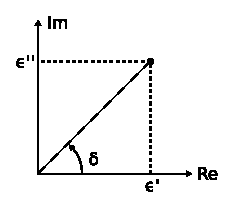
\includegraphics[width=0.8\columnwidth]{modules/m0132_fLossTan2.eps} 
% https://commons.wikimedia.org/wiki/File:Loss_tangent_definition.svg
}}{A point in the Re-Im plane has a real and imaginary component. The point is an angle small delta from the real axis. Real component is labeled small epsilon double prime and the imaginary component is small epsilon double prime.}
\end{center}
\centerline{\scriptsize 
\copyright~\hyperref[m0132_fLossTan2_Credit]{C.\ Wang} 
\href{https://creativecommons.org/licenses/by-sa/4.0/}{CC BY-SA 4.0} 
} 
\caption{
\label{m0132_fLossTan2}
Loss tangent defined in terms of the real and imaginary components of the complex permittivity $\epsilon_c$.
}
\end{figure}

The discussion in this section has assumed that $\epsilon_c$ is complex-valued solely due to ohmic loss. 
However, it is explained in Section~\ref{m0134_Complex_Permittivity} that permittivity may also be complex-valued as a way to model delay in the response of ${\bf D}$ to changing ${\bf E}$.
Does the concept of loss tangent apply also in this case?
Since the math does not distinguish between permittivity which is complex due to loss and permittivity which is complex due to delay, subsequent mathematically-derived results apply in either case.
On the other hand, there may be potentially significant differences in the physical manifestation of these effects.
For example, a material having large loss tangent due to ohmic loss might become hot when a large electric field is applied, whereas a material having large loss tangent due to delayed response might not.
Summarizing:
%
%%%%%%%%%%%%%%%%%%%%%%%%%%%%%%%%%%%%%%%%%%%%%%%
%ORB HIGHLIGHT
\begin{mdframed}[backgroundcolor=yellow!20,nobreak=true] 
The expression for loss tangent given by Equation~\ref{m0132_lt2} and Figure~\ref{m0132_fLossTan2} does not distinguish between ohmic loss and delayed response.
\end{mdframed}
%%%%%%%%%%%%%%%%%%%%%%%%%%%%%%%%%%%%%%%%%%%%%%%

~\\
%%%%%%%%%%%%%%%%%%%%%%%%%%%%%%%%%%%%%%%%%%%%%%%%%%%%%%%

{\bf Additional Reading:}
\begin{itemize}
\item ``\href{https://en.wikipedia.org/wiki/Dielectric_loss}{Dielectric loss}'' on Wikipedia.
\end{itemize}

\index{loss tangent|)}






